%\documentclass[journal,12pt,draftclsnofoot,onecolumn]{IEEEtran} %draftclsnofoot
%\documentclass[confl, draftclsnofoot]{IEEEtran}
%\documentclass[conference,onecolumn,draft]{IEEEtran}
\documentclass[conference, 12pt]{IEEEtran}
\usepackage{fancyhdr}
\usepackage{grffile}
\usepackage{color}
\usepackage{graphicx}
\usepackage{cite}
\usepackage{multicol}
% \usepackage{subcaption}
\usepackage{algorithm}
\usepackage{algpseudocode}
\usepackage{pifont}
\usepackage{siunitx}
\usepackage{flushend}
\usepackage{amsmath}

%\usepackage{setspace}
%\doublespacing
%\onecolumn
\begin{document}
%
% paper title
% can use linebreaks \\ within to get better formatting as desired
    \title{
        Minimal Viable Waterworld Agents:\\
        Experimenting with MultiAgent Reinforcement Learning
    }
%
%
% author names and IEEE memberships
% note positions of commas and nonbreaking spaces ( ~ ) LaTeX will not break
% a structure at a ~ so this keeps an author's name from being broken across
% two lines.
% use \thanks{} to gain access to the first footnote area
% a separate \thanks must be used for each paragraph as LaTeX2e's \thanks
% was not built to handle multiple paragraphs
%

    \author{Michael Hegerhorst}

% note the % following the last \IEEEmembership and also \thanks -
% these prevent an unwanted space from occurring between the last author name
% and the end of the author line. i.e., if you had this:
%
% \author{....lastname \thanks{...} \thanks{...} }
%                     ^------------^------------^----Do not want these spaces!
%
% a space would be appended to the last name and could cause every name on that
% line to be shifted left slightly. This is one of those "LaTeX things". For
% instance, "\textbf{A} \textbf{B}" will typeset as "A B" not "AB". To get
% "AB" then you have to do: "\textbf{A}\textbf{B}"
% \thanks is no different in this regard, so shield the last } of each \thanks
% that ends a line with a % and do not let a space in before the next \thanks.
% Spaces after \IEEEmembership other than the last one are OK (and needed) as
% you are supposed to have spaces between the names. For what it is worth,
% this is a minor point as most people would not even notice if the said evil
% space somehow managed to creep in.


% The paper headers
%\markboth{Journal of \LaTeX\ Class Files,~Vol.~6, No.~1, January~2007}%
%{Shell \MakeLowercase{\textit{et al.}}: Bare Demo of IEEEtran.cls for Journals}
% The only time the second header will appear is for the odd numbered pages
% after the title page when using the twoside option.
%
% *** Note that you probably will NOT want to include the author's ***
% *** name in the headers of peer review papers.                   ***
% You can use \ifCLASSOPTIONpeerreview for conditional compilation here if
% you desire.


% If you want to put a publisher's ID mark on the page you can do it like
% this:
%\IEEEpubid{0000--0000/00\$00.00~\copyright~2007 IEEE}
% Remember, if you use this you must call \IEEEpubidadjcol in the second
% column for its text to clear the IEEEpubid mark.


% use for special paper notices
%\IEEEspecialpapernotice{(Invited Paper)}


% make the title area
    \maketitle
%copyright notice
% TODO
% \thispagestyle{plain}
% \fancypagestyle{plain}{
%   \fancyhf{} % clear all header and footer fields
%   \fancyfoot[L]{978-1-4673-8988-4/17/\$31.00~\copyright2017~IEEE} % change
%       copyright notice here if required
%   \renewcommand{\headrulewidth}{0pt}
%   \renewcommand{\footrulewidth}{0pt}
% }

    \begin{abstract}
        Reinforcement learning is a powerful tool that can be used to solve many problems.
These problems can range from extremely simple to extremely complex, and the agents
developed to solve these problems can be just as complex.
There is a need to develop agents that are complex enough to solve a given problem,
but simple enough so they do not require a large amount of resources.
This work makes the use of reinforcement learning agents in a well known
environment, known as Waterworld, and explores the effects of varying the complexity
of the agents.
Multiple algorithms are used to develop these agents, including Q-learning and
Actor-Critic models.
Similarly, the input received by the agents is changed in an attempt to build agents
that still work well, but require less resources.
% TODO: Fill in what is discovered

    \end{abstract}


% IEEEtran.cls defaults to using nonbold math in the Abstract.
% This preserves the distinction between vectors and scalars. However,
% if the journal you are submitting to favors bold math in the abstract,
% then you can use LaTeX's standard command \boldmath at the very start
% of the abstract to achieve this. Many IEEE journals frown on math
% in the abstract anyway.

% Note that keywords are not normally used for peerreview papers.
    \renewcommand\IEEEkeywordsname{Key Words}
    \begin{IEEEkeywords}
% TODO
% Synthetic biology, self organization, vascular development, tissue engineering,
%         genetic algorithms, optimization, bioengineering.
    \end{IEEEkeywords}

% For peer review papers, you can put extra information on the cover
% page as needed:
% \ifCLASSOPTIONpeerreview
% \begin{center} \bfseries EDICS Category: 3-BBND \end{center}
% \fi
%
% For peerreview papers, this IEEEtran command inserts a page break and
% creates the second title. It will be ignored for other modes.
%\IEEEpeerreviewmaketitle

    \section{Introduction}\label{sec:introduction}
% What and why
% Problem statement
% Given: find: such that: (solving a problem)
% Question if a methodological study

    \section{Methods}\label{sec:methods}
% RL method applied
% Experimental methods, (independent variables, dependent variables, control variables)


    \section{Results}\label{sec:results}

\subsection{Agent Type}\label{subsec:agent-type}
The average rewards by agent type can be seen in \autoref{fig:rewards-by-agent}.
Unfortunately, none of the agents were able to do as well as the controller used by the
CPT\@.
Additionally, all agents performed as bad or worse as a simple random controller!
It is possible that this problem is complex enough that the models needed more time
to train, but no significant additional gains were made when training for over 12,000
episodes, so there appears to be something wrong.

\begin{figure}[!ht]
    \centering
    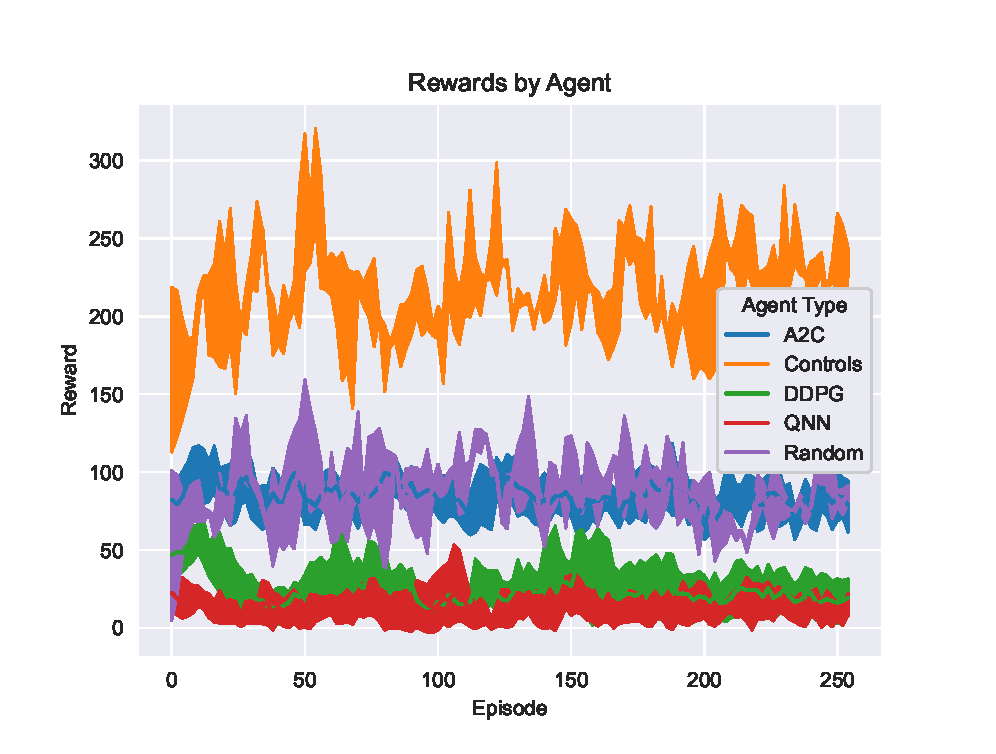
\includegraphics[scale=0.5]
    {./figures/rewards-by-agent}
    \caption{
        Rewards by agent type.
        The x-axis is the episode, while the y-axis is the reward.
    }
    \label{fig:rewards-by-agent}
\end{figure}

Interestingly, the A2C agents seems to perform the best out of all the agents used.
DDPG seems to perform second best, while QNN performs the worst.
Further work should be done to determine why these agents aren't improving and what
changes need to be made to improve them.
The average reward for each agent is shown in \autoref{tab:agent-average-reward}.

\begin{table}[!htbp]
    % increase table row spacing, adjust to taste
    \renewcommand{\arraystretch}{1.3}

    \caption{The average rewards by agent type.}
    \label{tab:agent-average-reward}

    \centering
    \begin{tabular}{|c|c|}
        \hline
        Agent    & Average Reward \\
        \hhline{|=|=|}
        A2C      & 84.767738      \\
        \hline
        Controls & 216.745977     \\
        \hline
        DDPG     & 25.048716      \\
        \hline
        QNN      & 13.036532      \\
        \hline
        Random   & 87.680823      \\
        \hline
    \end{tabular}
\end{table}

\subsection{Memory Type}\label{subsec:memory-type}
test

\begin{figure}[!ht]
    \centering
    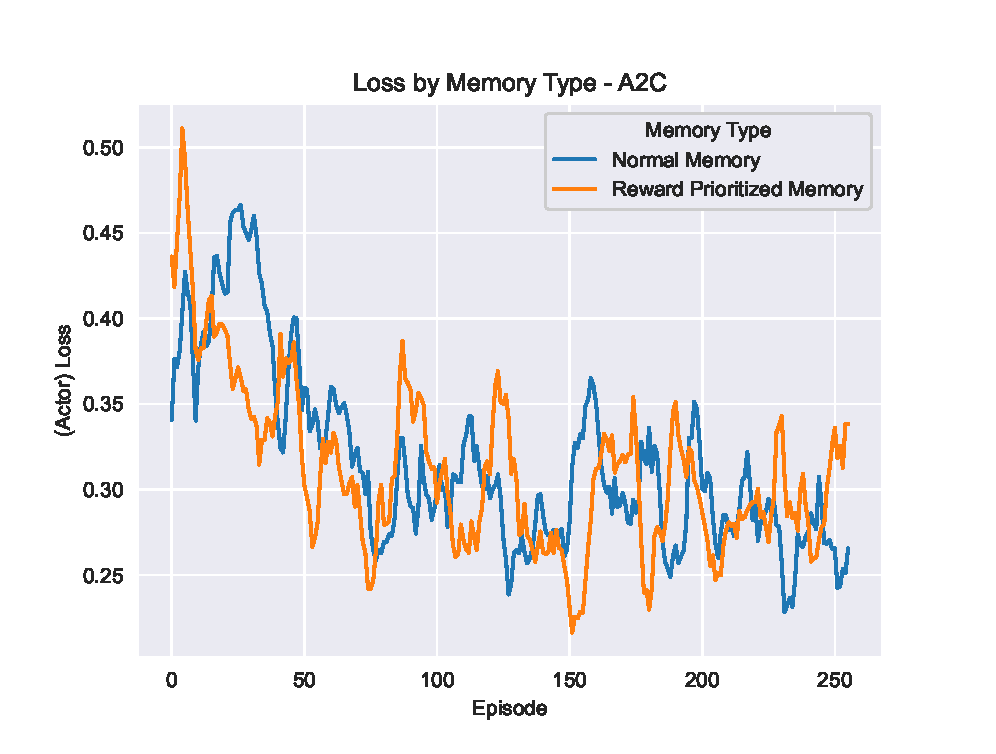
\includegraphics[scale=0.5]
    {./figures/memory/loss-by-memory-A2C}
    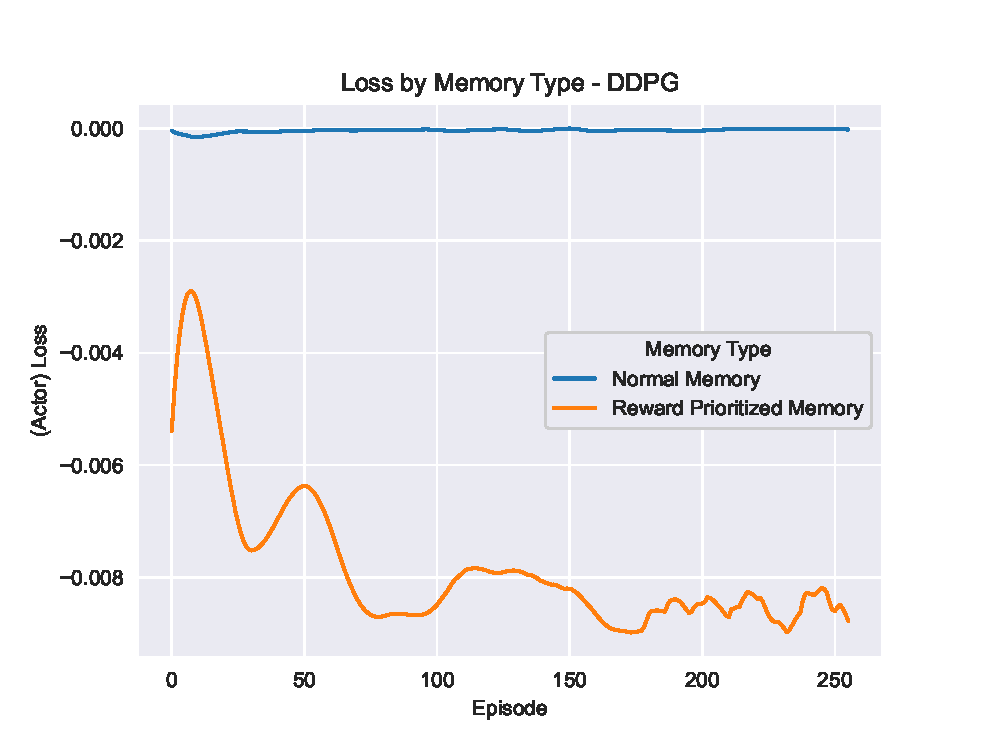
\includegraphics[scale=0.5]
    {./figures/memory/loss-by-memory-DDPG}
    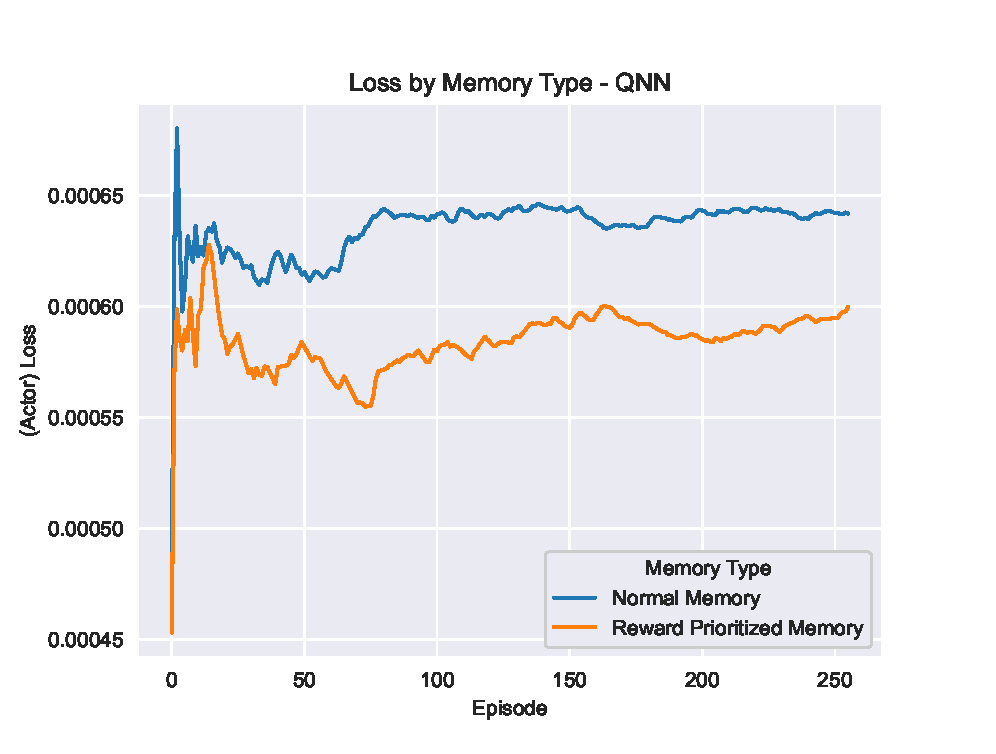
\includegraphics[scale=0.5]
    {./figures/memory/loss-by-memory-QNN}
    \caption{
        Rewards by agent type.
        The x-axis is the episode, while the y-axis is the reward.
    }
    \label{fig:loss-by-memory}
\end{figure}

test

\subsection{Architecture}\label{subsec:architecture}

\subsection{DDPG with CPT}\label{subsec:ddpg-with-cpt}

    \input{content/summary}
    \section{Conclusions}\label{sec:conclusions}
We have experimented with multiple agent architectures, including Distance and Simple
networks, as well as types of agents such as Q-learning, A2C, and DDPG\@.
We additionally developed and tested special training techniques including Controls
Policy Trainer and Reward Prioritized Memory.

We discovered all of these algorithms seem to struggle to adapt to Waterworld, but
A2C appears to perform best.
As previously shown, imitation learning can benefit agents learning Waterworld and
may be a more viable option.
However, we also were able to show there may be potential in using CPT, and encourage
additional research into how CPT can be used to enhance the DDPG and other training
algorithms.

    % TODO
    % Sources
    %   Citations to papers
    %   Links to websites
    %   Code sources
    %   How to publish, link to your own webpage, git hub page, etc.

    \bibliographystyle{plain}

    \begin{small}

        \bibliography{references}

    \end{small}


\end{document}
